\subsection{Results and Analysis}

In the following sections, results from each method discussed in chapter \ref{clustering_methods} are shown and described.
The scores used in this chapter are from our notebook experiments as we worked with them for the majority of the project duration and are thus most familiar with them. Results from the main clustering pipeline with similar parameters can and will differ slightly.

\subsubsection{LDA and LSA}
\subsubcomment{Written by Jessica Kaechele}
By using the topic modeling methods LSA and LDA, first insights into the nature of the data can be gained.

Table \ref{tab:lda_lsa_topwords} shows the top words when forming two clusters using LDA and LSA.
\begin{table}[]
    \centering
    \caption{Top words of two clusters retrieved by LDA and LSA}
    \begin{tabular}{l|l|l|l}
        \multicolumn{2}{c}{LDA} & \multicolumn{2}{c}{LSA} \\
        Cluster 1 & Cluster 2 & Cluster 1 & Cluster 2\\
        \hline
        \shortstack[l]{alexey \\ bibliography \\ chervonenkis \\ preface \\ synergy \\ comment \\ deap \\ repeating \\ manopt \\ introductory} & \shortstack[l]{model \\ learning \\ algorithm \\ data \\ method \\ problem \\ function \\ matrix \\ kernel \\ regression} & \shortstack[l]{model \\ graph \\ network \\ graphical \\ inference \\ latent \\ causal \\ data \\ variable \\ gaussian} & \shortstack[l]{model \\ algorithm \\ learning \\ data \\ method \\ problem \\ function \\ matrix \\ kernel \\ regression} 
    \end{tabular}
    \label{tab:lda_lsa_topwords}
\end{table}
While the terms describing cluster 2 are very general, those of cluster 1 are very specific.
In the case of LDA, they even include names.
This indicates that many papers are assigned to cluster 2 and only a few to cluster 1.
This can also be observed when extracting more than two clusters.
The visualization in 2 dimensions, which can be seen in figure \ref{fig:lda_lsa}, strengthens this assumption.
\begin{figure}
\centering
\begin{subfigure}{.4\textwidth}
  \centering
  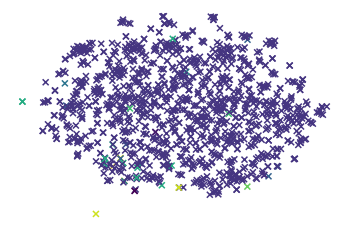
\includegraphics[width=\linewidth]{imgs/lda.png}
  \caption{LDA}
  \label{fig:lda}
\end{subfigure}%
\begin{subfigure}{.4\textwidth}
  \centering
  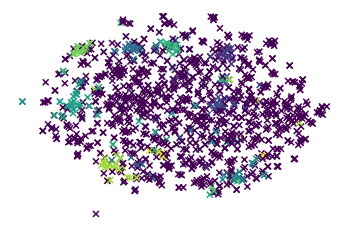
\includegraphics[width=\linewidth]{imgs/lsa.png}
  \caption{LSA}
  \label{fig:lsa}
\end{subfigure}
\caption{two-dimensional representation of 15 clusters}
\label{fig:lda_lsa}
\end{figure}
In the case of LDA, a large proportion of the papers are assigned to one cluster, while other culsters appear only rarely.
With LSA, a few small clusters can be identified, but these are located within a large cluster.

These results are also found in the evaluation metrics, as can be seen in table \ref{tab:scores_lsa_lda}.
\begin{table}[]
    \centering
    \begin{tabular}{c|c|c|c}
     Model & Silhouette Score & Calinski-Harabasz-Score & Davies-Bouldin-Score  \\
     \hline
     \hline
     LDA & -0.0026 & 1.1233 & 2.6217 \\
     \hline
     LSA & -0.0089 & 2.9692 & 4.4138
    \end{tabular}
    \caption{Metrics retrieved with LSA and LDA extracting 15 clusters}
    \label{tab:scores_lsa_lda}
\end{table}
The Calinski-Harabsz-Score is very low and the Silhouette Score is even negative.
The reason for this could be that the clusters are not clearly separated from each other.
The Davies-Bouldin-Score, however, seems to indicate better results, especially for LDA.
The reason for this could be that a cluster sometimes only consists of one paper and therefore the average distance between each point of the cluster and its cluster center is very low.

Both the metrics and the visual representation suggest that LSA and LDA are not suitable clustering algorithms for our data.


\subsubsection{K-Means}\label{subsubsec:kmeans}
\subsubcomment{Written by Jessica Kaechele}
Before clustering with K-Means, it is necessary to find a suitable number of clusters using the Elbow Method.
In figure \ref{fig:elbow} it can be seen that no kink is formed and therefore the number of clusters cannot be determined.
\begin{figure}
    \centering
    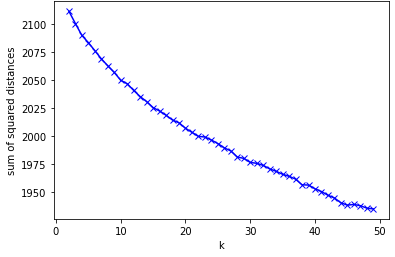
\includegraphics[width=0.5\linewidth]{imgs/elbow.png}
    \caption{Elbow Method with K-Means}
    \label{fig:elbow}
\end{figure}
The reason for this can be clearly seen in figure \ref{fig:kmeans_no_dim}.
\begin{figure}
\centering
\begin{subfigure}{.3\textwidth}
    \centering
    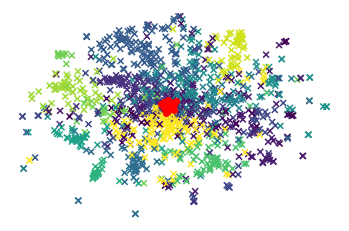
\includegraphics[width=\linewidth]{imgs/kmeans.png}
    \caption{No dimensionality reduction}
    \label{fig:kmeans_no_dim}
\end{subfigure}
\begin{subfigure}{.3\textwidth}
  \centering
  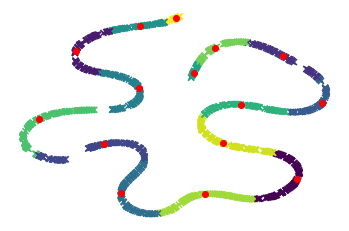
\includegraphics[width=\linewidth]{imgs/kmeans_lsa.png}
  \caption{LSA}
  \label{fig:kmeans_lsa}
\end{subfigure}%
\begin{subfigure}{.3\textwidth}
  \centering
  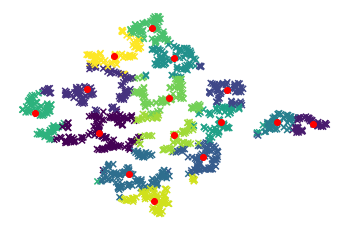
\includegraphics[width=\linewidth]{imgs/kmeans_spectral.png}
  \caption{Spectral Embedding}
  \label{fig:kmeans_spectral}
\end{subfigure}
\caption{two-dimensional representation of 15 clusters retrieved by K-Means with their centroids with different dimensionality reductions}
\label{fig:kmeans}
\end{figure}
Because a cluster contains fewer data points the more clusters have formed the sum of squared distances becomes smaller.
But an ideal value for $k$ does not arise, because of the centroids which are all located exactly in the center of the dataset.

If a dimensionality reduction using LSA or Spectral Embedding is applied before clustering, an elbow can be seen.
The data is reduced to two components, with both dimensionality reduction methods, since it leads to the best scores.
Additionally, the optimal number of clusters seems to be 15 since the elbow flattens at this point.
The scores improve significantly compared to K-Means without dimensionality reduction as can be seen in table \ref{tab:scores_kmeans}.
\begin{table}[]
    \centering
    \begin{tabular}{c|c|c|c}
     Model &  \shortstack[c]{Silhouette \\ Score} & \shortstack[c]{Calinski-Harabasz \\ Score} &  \shortstack[c]{Davies-Bouldin \\ Score}  \\
     \hline
     \hline
     K-Means & 0.0103 & 7.303 & 7.7293 \\
     \hline
     \shortstack[c]{K-Means with \\ LSA} & 0.521 & 16793.344 & 0.53472 \\
     \hline
     \shortstack[c]{K-Means with \\ Spectral Embedding} & 0.3402 & 1813.0376 & 0.834 \\
     \hline
     \shortstack[c]{K-Means \\ with LSA and \\ custom stopword removal} & 0.5336 & 14589.2349 & 0.5109 \\

    \end{tabular}
    \caption{Metrics retrieved with K-Means extracting 15 clusters}
    \label{tab:scores_kmeans}
\end{table}
Visually, clusters are now clearly visible and the cluster centroids are better distributed.
This can be seen in figure \ref{fig:kmeans}.

It can be observed that terms like \textit{algorithm}, \textit{method}, \textit{data} appear in the top words of many clusters.
By removing these words, it might be possible to separate the clusters even better. 
But it turns out, that although these terms no longer appear, other terms do show up, which appear in many clusters.
Besides, the metrics in table \ref{tab:scores_kmeans} show that the clusters hardly change.
Only the Calinski-Harabasz-Score deteriorates significantly. This indicates that the clusters are now no longer as dense or easily separable.


\subsubsection{Spectral Clustering}
\subsubcomment{Written by Jessica Kaechele}
Since Spectral Clustering consists of Spectral Embedding and K-Means, it should yield similar results to those obtained in section \ref{subsubsec:kmeans}.
However, this is not the case.
The Silhouette Score is only $0.0117$, the Calinski-Harabasz-Score is $4.57$ and the Davies-Bouldin-Score is $6.518$.
If one compares these values with the results obtained using Spectral Embedding and K-Means (see table \ref{tab:scores_kmeans}), it can be seen that the results are significantly worse.
The reason for this could be different parameters.
However, even after using the same parameters in both approaches, it is not possible to achieve similarly good results. 
Another reason could be that in the sklearn implementation the \textit{drop\_first} parameter is False.
But why the results are so different needs further investigation.



\subsubsection{BIRCH}
\subsubcomment{Written by Jessica Kaechele}
Similar to K-Means, BIRCH combined with a dimensionality reduction achieves better results, as can be seen in table \ref{tab:scores_birch}.
\begin{table}[]
    \centering
    \begin{tabular}{c|c|c|c}
     Model &  \shortstack[c]{Silhouette \\ Score} & \shortstack[c]{Calinski-Harabasz \\ Score} &  \shortstack[c]{Davies-Bouldin \\ Score}  \\
     \hline
     \hline
     BIRCH & 0.0017 & 4.056 & 6.8339 \\
     \hline
     \shortstack[c]{BIRCH with \\ LSA} & 0.4852 & 6294.5856 & 0.4793
 \\
     \hline
     \shortstack[c]{BIRCH with \\ Spectral Embedding} & 0.3238 & 1007.1024 & 0.8867 \\
     \hline
     \shortstack[c]{BIRCH \\ with LSA and \\ custom stopword removal} & 0.4984 & 7511.1226 & 0.8867 \\

    \end{tabular}
    \caption{Metrics retrieved with BIRCH extracting 15 clusters}
    \label{tab:scores_birch}
\end{table}
This can also be seen in the two-dimensional representation(see figure \ref{fig:birch}) where the clusters look well separated with LSA and Spectral Embedding.
\begin{figure}
\centering
\begin{subfigure}{.3\textwidth}
    \centering
    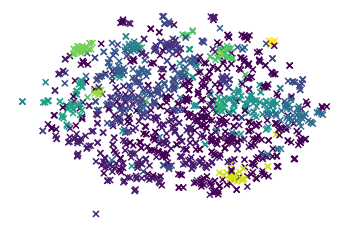
\includegraphics[width=\linewidth]{imgs/birch.png}
    \caption{No dimensionality reduction}
    \label{fig:birch_no_dim}
\end{subfigure}
\begin{subfigure}{.3\textwidth}
  \centering
  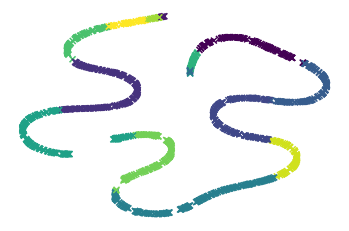
\includegraphics[width=\linewidth]{imgs/birch_lsa.png}
  \caption{LSA}
  \label{fig:birch_lsa}
\end{subfigure}%
\begin{subfigure}{.3\textwidth}
  \centering
  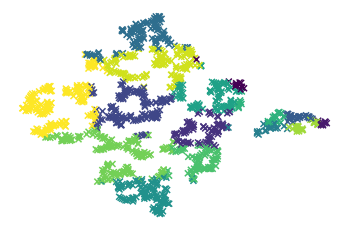
\includegraphics[width=\linewidth]{imgs/birch_spectral.png}
  \caption{Spectral Embedding}
  \label{fig:birch_spectral}
\end{subfigure}
\caption{two-dimensional representation of 15 clusters retrieved by BIRCH with different dimensionality reductions}
\label{fig:birch}
\end{figure}
In addition, the best results are also achieved by using two components.
But the optimal number of clusters cannot be determined using the Elbow Method because the cluster centroids are not known.
Instead, the Silhouette Score, Calinski-Harabasz-Score, and Davies-Bouldin-Score are used.
It turns out that, similar to K-Means, 10 to 15 clusters are ideal.

The stopword removal of words that occur in many clusters shows that the composition of the cluster changes a little here.
The decreasing Davies-Bouldin-Score implies that the separation between two clusters is slightly worsened by the removal, while the increasing Calinski-Harabasz-Score indicates that the clusters are slightly denser.
However, whether the clustering improves by the removal is difficult to say with the scores.

\subsubsection{Affinity Propagation}
\subsubcomment{Written by Jonas Reinwald}

As with most of the tested clustering methods, using some kind of dimensionality reduction significantly increases all metrics. As can be seen in table \ref{tab:scores_affinity_propagation} scores without dimensionality reduction are very poor.
In these cases Affinity Propagation produced a lot of clusters, most of them containing very similar data. This is also evident in figure \ref{fig:affinity_propagation}, where the first plot shows no clear clusters at all. In contrast, the two subplots with LSA and Spectral Embedding show better clustering, albeit with still quite some overlap. 

\begin{table}[]
  \centering
  \begin{tabular}{c|c|c|c}
    Model &  \shortstack[c]{Silhouette \\ Score} & \shortstack[c]{Calinski-Harabasz \\ Score} &  \shortstack[c]{Davies-Bouldin \\ Score}  \\
    \hline
    \hline
    Affinity Propagation & 0.030495 & 2.134269 & 2.853512 \\
    \hline
    \shortstack[c]{Affinity Propagation with \\ LSA} & 0.193265 & 180.728882 & 1.26669 \\
    \hline
    \shortstack[c]{Affinity Propagation with \\ Spectral Embedding} & 0.188029 & 199.463342 & 1.30149 \\
    \hline
    \shortstack[c]{Affinity Propagation with \\ custom stopword removal} & 0.031234 & 2.141206 & 2.839059 \\
   \end{tabular}
  \caption{Metrics retrieved with Affinity Propagation}
  \label{tab:scores_affinity_propagation}
\end{table}

\begin{figure}
  \centering
  \begin{subfigure}{.3\textwidth}
      \centering
      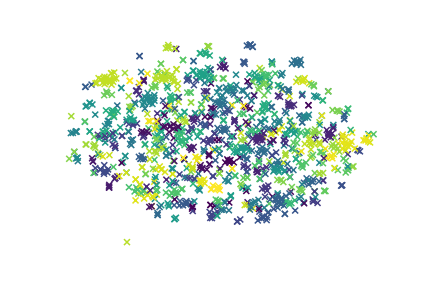
\includegraphics[width=\linewidth]{imgs/affinity_propagation.png}
      \caption{No dimensionality reduction}
      \label{fig:affinity_propagation_no_dim}
  \end{subfigure}
  \begin{subfigure}{.3\textwidth}
    \centering
    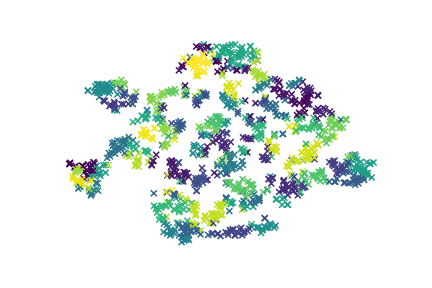
\includegraphics[width=\linewidth]{imgs/affinity_propagation_lsa.png}
    \caption{LSA}
    \label{fig:affinity_propagation_lsa}
  \end{subfigure}%
  \begin{subfigure}{.3\textwidth}
    \centering
    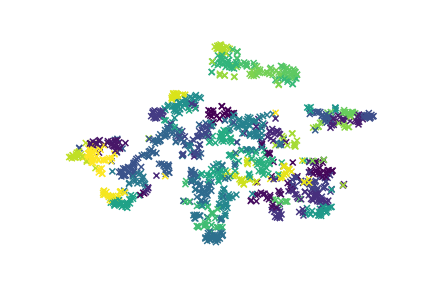
\includegraphics[width=\linewidth]{imgs/affinity_propagation_spectral.png}
    \caption{Spectral Embedding}
    \label{fig:affinity_propagation_spectral}
  \end{subfigure}
  \caption{Two-dimensional representation of clusters retrieved by Affinity Propagation with different dimensionality reduction methods}
  \label{fig:affinity_propagation}
\end{figure}

\subsubsection{Agglomerative Clustering}
\subsubcomment{Written by Jonas Reinwald}

As with Affinity Propagation, Agglomerative Clustering shows the same pattern for scores. In comparison with the former and shown in table \ref{tab:scores_agglomerative}, clustering on the raw pre-processed data produces a better Calinski-Harabasz Index, indicating slightly denser clusters, but a worse Davies-Bouldin Index, indicating less separation between clusters.
Using dimensionality reduction improves all metrics by a large margin, with LSA having one of the best scores overall. Figure \ref{fig:agglomerative} visually confirms this, with Spectral Embedding showing some perceivable distinction and LSA showing almost perfect distinction between clusters.

\begin{table}[]
  \centering
  \begin{tabular}{c|c|c|c}
    Model &  \shortstack[c]{Silhouette \\ Score} & \shortstack[c]{Calinski-Harabasz \\ Score} &  \shortstack[c]{Davies-Bouldin \\ Score}  \\
    \hline
    \hline
    Agglomerative Clustering & 0.000467 & 4.084053 & 6.231226 \\
    \hline
    \shortstack[c]{Agglomerative Clustering with \\ LSA} & 0.512373 & 10238.480445 & 0.509119 \\
    \hline
    \shortstack[c]{Agglomerative Clustering with \\ Spectral Embedding} & 0.300136 & 1029.213757 & 0.904163 \\
    \hline
    \shortstack[c]{Agglomerative Clustering with \\ custom stopword removal} & 0.001866 & 4.153627 & 6.278349 \\
   \end{tabular}
  \caption{Metrics retrieved with Agglomerative Clustering}
  \label{tab:scores_agglomerative}
\end{table}

\begin{figure}
  \centering
  \begin{subfigure}{.3\textwidth}
      \centering
      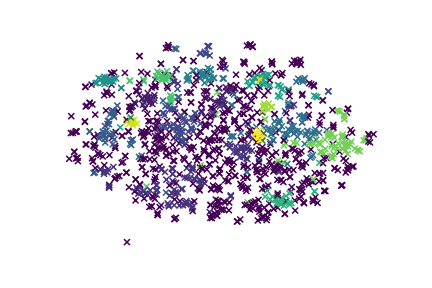
\includegraphics[width=\linewidth]{imgs/agglomerative.png}
      \caption{No dimensionality reduction}
      \label{fig:agglomerative_no_dim}
  \end{subfigure}
  \begin{subfigure}{.3\textwidth}
    \centering
    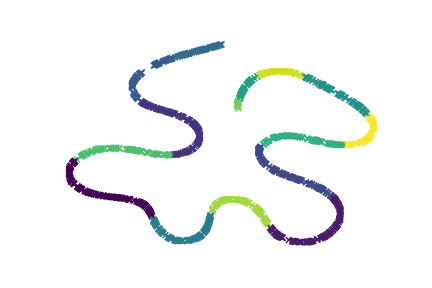
\includegraphics[width=\linewidth]{imgs/agglomerative_lsa.png}
    \caption{LSA}
    \label{fig:agglomerative_lsa}
  \end{subfigure}%
  \begin{subfigure}{.3\textwidth}
    \centering
    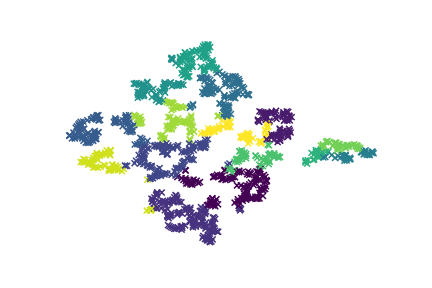
\includegraphics[width=\linewidth]{imgs/agglomerative_spectral.png}
    \caption{Spectral Embedding}
    \label{fig:agglomerative_spectral}
  \end{subfigure}
  \caption{Two-dimensional representation of clusters retrieved by Agglomerative Clustering with different dimensionality reduction methods}
  \label{fig:agglomerative}
\end{figure}

\subsubsection{DBSCAN}
\subsubcomment{Written by Jonas Reinwald}

DBSCAN did not yield any desirable results at all. As can be seen in table \ref{tab:scores_dbscan} scores without dimensionality reduction are just as bad as with other methods and scored with dimensionality reduction are missing completely. This is because in our experiments almost all parameter settings produced only one single big cluster for normal data and one single big cluster for all tested parameter settings with LSA or Spectral Embedding, making score calculation impossible.
This is also the reason why all data points in figure \ref{fig:dbscan}, except for a few in the first subplot, are colored the same.

Because of the data-dependent threshold value (see section \ref{subsubsec:dbscan}), it might be possible to achieve better clustering by testing even more parameter values or using some kind of heuristic to find appropriate values.

\begin{table}[]
  \centering
  \begin{tabular}{c|c|c|c}
    Model &  \shortstack[c]{Silhouette \\ Score} & \shortstack[c]{Calinski-Harabasz \\ Score} &  \shortstack[c]{Davies-Bouldin \\ Score}  \\
    \hline
    \hline
    DBSCAN & -0.009707 & 2.061513 & 1.887693 \\
    \hline
    \shortstack[c]{DBSCAN with \\ custom stopword removal} & -0.010665 & 2.052975 & 1.890026 \\
   \end{tabular}
  \caption{Metrics retrieved with DBSCAN}
  \label{tab:scores_dbscan}
\end{table}

\begin{figure}
  \centering
  \begin{subfigure}{.3\textwidth}
      \centering
      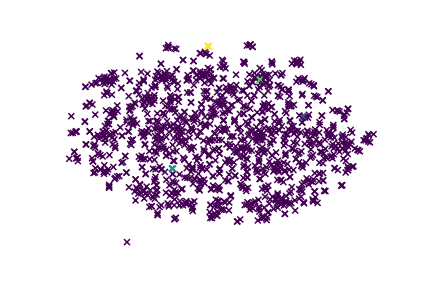
\includegraphics[width=\linewidth]{imgs/dbscan.png}
      \caption{No dimensionality reduction}
      \label{fig:dbscan_no_dim}
  \end{subfigure}
  \begin{subfigure}{.3\textwidth}
    \centering
    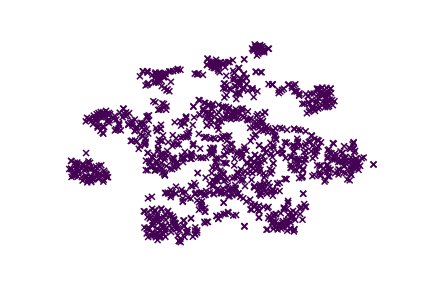
\includegraphics[width=\linewidth]{imgs/dbscan_lsa.png}
    \caption{LSA}
    \label{fig:dbscan_lsa}
  \end{subfigure}%
  \begin{subfigure}{.3\textwidth}
    \centering
    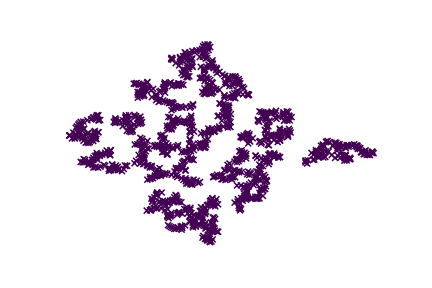
\includegraphics[width=\linewidth]{imgs/dbscan_spectral.png}
    \caption{Spectral Embedding}
    \label{fig:dbscan_spectral}
  \end{subfigure}
  \caption{Two-dimensional representation of clusters retrieved by DBSCAN with different dimensionality reduction methods}
  \label{fig:dbscan}
\end{figure}

\subsubsection{OPTICS}
\subsubcomment{Written by Jonas Reinwald}

\begin{table}[]
  \centering
  \begin{tabular}{c|c|c|c}
    Model &  \shortstack[c]{Silhouette \\ Score} & \shortstack[c]{Calinski-Harabasz \\ Score} &  \shortstack[c]{Davies-Bouldin \\ Score}  \\
    \hline
    \hline
    OPTICS & -0.003231 & 2.455650 & 2.620644 \\
    \hline
    \shortstack[c]{OPTICS with \\ LSA} & 0.346423 & 41.642624 & 1.53435 \\
    \hline
    \shortstack[c]{OPTICS with \\ Spectral Embedding} & -0.191176 & 13.449457 & 1.788995 \\
    \hline
    \shortstack[c]{OPTICS with \\ custom stopword removal} & -0.004380 & 2.567746 & 2.628210 \\
   \end{tabular}
  \caption{Metrics retrieved with OPTICS}
  \label{tab:scores_optics}
\end{table}

\begin{figure}
  \centering
  \begin{subfigure}{.3\textwidth}
      \centering
      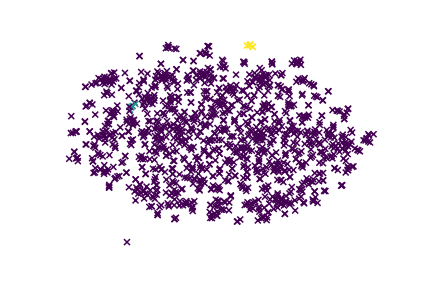
\includegraphics[width=\linewidth]{imgs/optics.png}
      \caption{No dimensionality reduction}
      \label{fig:optics_no_dim}
  \end{subfigure}
  \begin{subfigure}{.3\textwidth}
    \centering
    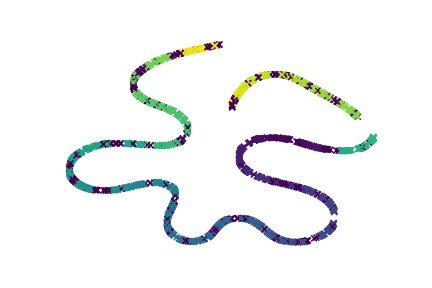
\includegraphics[width=\linewidth]{imgs/optics_lsa.png}
    \caption{LSA}
    \label{fig:optics_lsa}
  \end{subfigure}%
  \begin{subfigure}{.3\textwidth}
    \centering
    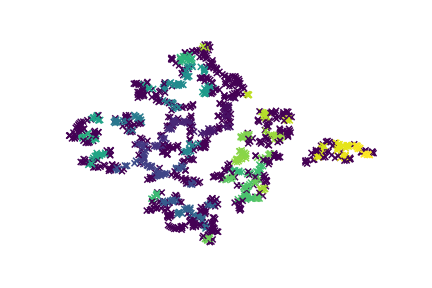
\includegraphics[width=\linewidth]{imgs/optics_spectral.png}
    \caption{Spectral Embedding}
    \label{fig:optics_spectral}
  \end{subfigure}
  \caption{Two-dimensional representation of clusters retrieved by OPTICS with different dimensionality reduction methods}
  \label{fig:optics}
\end{figure}

\subsubsection{MeanShift}
\subsubcomment{Written by Jonas Reinwald}

\begin{table}[]
  \centering
  \begin{tabular}{c|c|c|c}
    Model &  \shortstack[c]{Silhouette \\ Score} & \shortstack[c]{Calinski-Harabasz \\ Score} &  \shortstack[c]{Davies-Bouldin \\ Score}  \\
    \hline
    \hline
    \shortstack[c]{MeanShift with \\ LSA} & 0.410777 & 2443.830097 & 0.543272 \\
    \hline
    \shortstack[c]{MeanShift with \\ Spectral Embedding} & 0.474139 & 646.527661 & 0.799436 \\
   \end{tabular}
  \caption{Metrics retrieved with MeanShift}
  \label{tab:scores_mean_shift}
\end{table}

\begin{figure}
  \centering
  \begin{subfigure}{.3\textwidth}
      \centering
      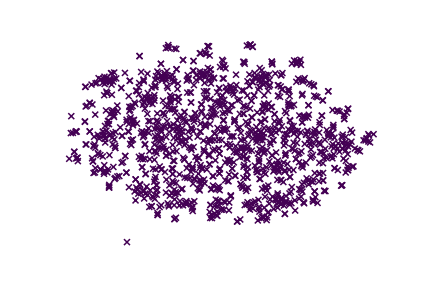
\includegraphics[width=\linewidth]{imgs/mean_shift.png}
      \caption{No dimensionality reduction}
      \label{fig:mean_shift_no_dim}
  \end{subfigure}
  \begin{subfigure}{.3\textwidth}
    \centering
    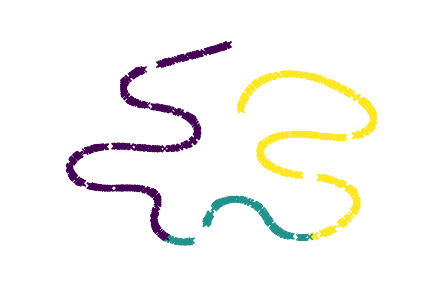
\includegraphics[width=\linewidth]{imgs/mean_shift_lsa.png}
    \caption{LSA}
    \label{fig:mean_shift_lsa}
  \end{subfigure}%
  \begin{subfigure}{.3\textwidth}
    \centering
    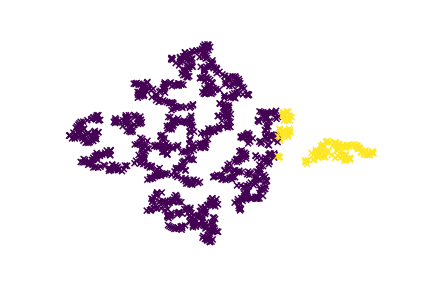
\includegraphics[width=\linewidth]{imgs/mean_shift_spectral.png}
    \caption{Spectral Embedding}
    \label{fig:mean_shift_spectral}
  \end{subfigure}
  \caption{Two-dimensional representation of clusters retrieved by MeanShift with different dimensionality reduction methods}
  \label{fig:mean_shift}
\end{figure}